% -*- mode: LaTeX; coding: utf8; -*-

\documentclass[a4paper,14pt]{extreport}

\usepackage[utf8]{inputenc}
\usepackage[english,ukrainian]{babel}
\usepackage[T1, T2A]{fontenc}
\usepackage{dsfont}
\usepackage[export]{adjustbox}

\usepackage{indentfirst}
\selectlanguage{ukrainian}

\usepackage{fontspec}
\setmainfont{Times New Roman}

% інтервал - півтора. 
\usepackage{setspace}
\onehalfspacing

% поля
\usepackage{geometry}
\geometry{a4paper}
\geometry{left=25mm,right=10mm,top=20mm,bottom=20mm}
\geometry{headheight=2ex,headsep=10mm,footskip=10mm}

%
\usepackage{mathtools}
\usepackage{mathrsfs, amsmath}


%для картинок
\usepackage{graphicx}
\usepackage{caption}

% lstlisting settings
\usepackage{xcolor}

% для часткових похідних
\usepackage{physics}

\usepackage{amssymb}

\usepackage{color}
\usepackage{listings}

\usepackage{algorithmicx}

\lstset{
	extendedchars=\true, % дозволити кирилицю в лінстингу
	inputencoding=utf8,
	breaklines=true,
	basicstyle=\ttfamily,
	numbers=left,
	frame=single,
	backgroundcolor=\color{bluegray}
}

% якщо прийдеться вставляти код (простіше ніж listings, але немає breaklines)
\usepackage{verbatim}

% для алгоритмів
%\usepackage[ruled,vlined]{algorithm2e}
\usepackage{algpseudocode}
\usepackage{algorithm}
\floatname{algorithm}{Algorithm}
\renewcommand{\algorithmicrequire}{\textbf{Input: }}
\renewcommand{\algorithmicensure}{\textbf{Output: }}
\newcommand{\algorithmreturn}{\textbf{return }}

% bibliography
\usepackage[
backend=biber,
style=numeric,
sorting=ynt
]{biblatex}
\addbibresource{resources/bibres.bib}

% custom commands
\newcommand{\tran}{^{T}}
\newcommand{\ith}{^{(i)}}

\begin{document}
	% ============================================ %
	\begin{titlepage}%
    	\begin{center}
	    	{\textbf{ЛЬВІВСЬКИЙ НАЦІОНАЛЬНИЙ УНІВЕРСИТЕТ \\ ІМЕНІ ІВАНА ФРАНКА}}\par
	       	{Факультет прикладної математики та інформатики \\ Кафедра обчислювальної математики}\par
			\begin{center}
	
	        \end{center}
	        \vspace{25mm}
	        {\textbf{\huge{Курсова робота}}}\par
	        \vspace{5mm}
	        {АНАЛІЗ АТАК НА ЛІНІЙНІ МОДЕЛІ МАШИННОГО НАВЧАННЯ}\par
	        \vspace{5mm}
	        {}\par %subtitle
        \end{center}
	   	
	   	\vspace{30mm}
	   	
		\begin{flushright}
   	   		\begin{minipage}[t]{107mm}
   	   			\flushleft{
   	   			{\large{
			   	   		Виконав: студент \underline{III} курсу групи \underline{ПМп-31} напрямку підготовки (спеціальності) \\
			   	   		113 $-$ "Прикладна математика" \hfill \\
				}}
	   	   	   	{\large{
	   	   	   			\noindent\underline{\makebox[107mm]{\hfill Середович В.В.}} \\
   	   	   		}}
      			{\small{
    					\hfill \footnotesize{(прізвище та ініціали)} \\
	   	   		}}
	   	   		{\large{
	   	   				Керівник: \noindent\underline{\makebox[80.3mm]{\hfill Музичук Ю.А.}}
	   	   		}}
      			} \\
	   	   		{\small{
			   	   		\hfill \footnotesize{(прізвище та ініціали)} \\
			   	   		\vspace{2ex}
				}}
   	   		\end{minipage}
   	   \end{flushright}
	   \vfill
   	   
   	   \begin{center}Львів --- 2020\end{center}
   	   \stepcounter{page}
    \end{titlepage}
	% ============================================ %
	\addtocontents{toc}{\protect\thispagestyle{empty}}
	\tableofcontents
	% ============================================ %
	\addcontentsline{toc}{section}{Вступ}
	\chapter*{Вступ}
	Алгоритми машинного навчання активно використовується у різних областях нашого життя та дуже добре демонструють себе у задачах класифікації. Однак, виявляється, що ці алгоритми є досить вразливими навіть до незначних, правильно підібраних, пертурбацій вхідної інформації. Такі модифіковані приклади, які навмисно змінюють для того, щоб вони були хибно передбаченні називають змагальними прикладами або adversarial samples. В деяких випадках ці зміни можуть бути настільки малі, що для людини вони зовсім не будуть помітні, однак класифікатор моделі буде робити хибне передбачення. Така вразливість може бути дуже небезпечною коли алгоритми машинного навчання застосовуються в критичних для здоров'я людини задачах, таких як передбачення небезпечного захворювання або розпізнавання знаків дорожнього руху автопілотом машини. Саме тому, тема вразливостей алгоритмів машинного навчання та відповідних методів захисту які могли б запобігти небажаним наслідкам, привертає до себе багато уваги і потребує досліджень.
	
	В межах теми цієї роботи будемо розглядати декілька різних методів атак на лінійні моделі машинного навчання, які аналізуватимемо та порівнюватимемо між собою. Окрім того, також реалізуємо і перевіримо декілька методів захисту для того щоб визначити їх ефективність у захисті моделі. 
	% ============================================ %

	\chapter{Постановка задачі} 
	Метою даної роботи є дослідження ефективності різних методів атак на лінійні моделі машинного навчання, та аналіз можливих методів захисту від них.
	
	Виходячи з мети, визначеними завданнями роботи є:
	\begin{itemize}
	\item Реалізувати лінійну модель машинного навчання
	\item Розглянути різні методи генерування змагальних прикладів
	\item Застосувати атаки на створену модель та проаналізувати їх ефективність
	\item Розглянути можливі методи захисту від атак
	\end{itemize}
	
	\section{Основні поняття}	
	В цій секції будуть розглянуті основні терміни, які будуть використовуватись в ході роботи.
	
	\textbf{Змагальний приклад (Adversarial sample)}
	\newline
	Нехай існує класифікатор $f(x):x\rightarrow y$, де  $x \in X, y \in Y$, який передбачає значення $y$ для вхідного $x$. Метою змагального прикладу є знайти такий $x^{*}$, який знаходиться в околі $x$, але хибно визначається класифікатором. Зазвичай максимальний рівень шуму в змагальному прикладі може бути не більше за певну $L_p$ норму $ \| x^{*} - x \|_p < \varepsilon $, де $p=1,2,\infty $. В межах даної роботи для визначення рівня пертурбації буде використовуватись саме $L_{\infty}$ норма.
	\newline \par
	\textbf{Цілеспрямовані атаки (Targeted Attacks)} \newline
	Цілеспрямованими атаками є атаки, метою яких є внести в приклад $x$, який правильно передбачається як $f(x) = y$, незначний шум так, щоб класифікатор зробив хибне передбачення $f(x^{*}) \neq y$.
	\newline \par
	\textbf{Нецілеспрямовані  атаки (Untargeted Attacks)} \newline
	Нецілеспрямованими атаками називають такі атаки, метою яких є внести у вхідний приклад $x$ такі пертурбації, щоб класифікатор передбачив якийсь конкретний клас $f(x^{*}) = y^{*}$, де $y^{*}$ є заданою ціллю $y^{*} \neq y$.
	\newline \par
	\textbf{Атаки на відкриту модель (White Box attacks)} \newline
	Атаки на закриту модель описують такий сценарій, коли в нападника є повний доступ до внутрішніх параметрів моделі таких як ваги і параметр зсуву.
	\newline \par
	\textbf{Атаки на закриту модель (Black Box attacks)} \newline
	До атак на відкриту модель відносять атаки, при яких в нападника нема доступу до внутрішніх параметрів моделі і для створення успішного нападу він може використовувати тільки передбачення моделі.

	% ============================================ %

	% ============================================ %
	\chapter{Модель}
	
	\section{Мультикласова логістична регресія}
	\label{sec:lg}
	Лінійним методом машинного навчання, на котрий будемо здійснювати атаки, буде використовуватись модифікований алгоритм логістичної регресії для мультикласової класифікації. \par
	Нехай маємо набір тренувальних даних:
	\begin{equation*}
		(x^{(1)}, y^{(1)}), \quad (x^{(2)}, y^{(2)}), \quad ... \quad ,(x^{(m)}, y^{(m)})
	\end{equation*}
	\begin{equation*}
		\quad
		%%%
		X =	
		\begin{bmatrix}
		\vdots  & \vdots  & & \vdots \\
		x^{(1)} & x^{(2)} &   \dots & x^{(m)}\\
		\vdots  & \vdots  & & \vdots
		\end{bmatrix}
		%%%
		\quad
		%%%
		x \in
		\begin{bmatrix}
		x_1   \\
		\dots \\
		x_n
		\end{bmatrix}
		\hspace{21 mm}
		%%%
	\end{equation*}
	\begin{equation*}
		\quad
		%%%
		Y =	
		\begin{bmatrix}
		\vdots  & \vdots  & & \vdots \\
		y^{(1)} & y^{(2)} &   \dots & y^{(m)}\\
		\vdots  & \vdots  & & \vdots
		\end{bmatrix}
		%%%
		\quad
		%%%
		y \in
		\begin{bmatrix}
		y_1   \\
		\dots \\
		y_C
		\end{bmatrix}
		\quad
		y_1, ..., y_C
		%%%
	\end{equation*}
	\newline
	$X$ - матриця в якої кожен стовпець є набором характеристик $i-$ого прикладу, \newline $i=1,\dots,m$ 
	\newline
	$Y$ - матриця класів в якої кожен стовпець це масив розмірності $C$, з одиницею на місті справжнього класу
	\newline
	$m$ - кількість прикладів
	\newline
	$n$ - кількість характеристик в кожному прикладі
	\newline
	$C$ - кількість класів
	\newline \newline
	Задача прикладу $x \in R^{n}$, знайти $\hat{y}=P(y = 1 \mid x), \quad 0 \leq \hat{y} \leq 1$
	\begin{center}
	%Шукатимемо у вигляді:
	$\hat{y} = softmax(\omega\tran x + b)$, \quad де $\omega \in R^{n}, b \in R$ - невідомі параметри
	\end{center}
	Функція активації матиме вигляд:
	\begin{equation}	
		softmax(z) = \frac{e^{z}}{\sum_{k=1}^{C} e_k^z}
	\end{equation}
	Для кожного прикладу з тренувального датасету потрібно обчислити:
	\begin{equation*}
		z\ith = \omega\tran x\ith + b, \; \textup{де} \; \hat{y}\ith = softmax(z_i) = \frac{e^{z_i}}{\sum_{k=1}^{C} e_k^z}, \; \textup{так щоб} \; \hat{y}\ith \approx y\ith
	\end{equation*}
	В якості функції втрати буде використовуватись функція кросс-ентропії:
	\begin{equation}
		\label{eq:cross-entropy}
	\xi(y\ith, x\ith) = -\sum_{j=1}^{C} y_j \log(\hat{y_j}) \\
	\end{equation}
	\begin{equation}
		\xi(Y, X) =\frac{1}{m} \sum_{i=1}^{m}\xi(y\ith, x\ith) = -\frac{1}{m} \sum_{i=1}^{m} \sum_{j=1}^{C} y_{j}\ith \log (\hat{y}_j\ith) = J(\omega, b)
	\end{equation}
	Задача полягає в тому щоб знайти параметри $w \in R^n_x, b\in R$ що мінімізують \newline функцію $J(\omega, b)$.
	Для цього будемо використовувати алгоритм градієнтного спуску який буде виглядати наступним чином \ref{alg:gradient_descent}.
	
	\begin{algorithm}
		\caption{Градієнтний спуск}
		\label{alg:gradient_descent}
		\begin{algorithmic}[1]
			\State \algorithmicrequire{Тренувальні дані $X, Y$, гіперпараметри: $N$, $\varepsilon$, $\alpha$}
			\State \algorithmicensure{ Оптимальні параметри моделі $\omega, b$}
			\State i = 0
			\While{ i $< N$ або ( $\|d\omega\| < \varepsilon$ та $\|db\| < \varepsilon$ )}
			\State $d\omega = \alpha \pdv{J(\omega, b)}{\omega}$
			\State $db = \alpha \pdv{J(\omega, b)}{b}$
			\State $\omega = \omega - d\omega$
			\State $b = b - db$
			\State i += 1
			\EndWhile
			\State \algorithmreturn{$\omega, b$}.
		\end{algorithmic}
	\end{algorithm}
	
	\section{Датасет}
	В якості тренувального датасету будемо використовувати MNIST базу даних яка складається з 60 тис. тренувальних та 10 тис. тестувальних зображень рукописних цифр \ref{fig:minist_dataset}. Розмір кожного із них складає $28 \times 28$, а значення їх пікселів знаходяться в проміжку $[0, 255]$. На основі неї будемо здійснюватись тренування моделі і аналіз методів атак та захисту.
	\begin{figure}[h]
		\centering
		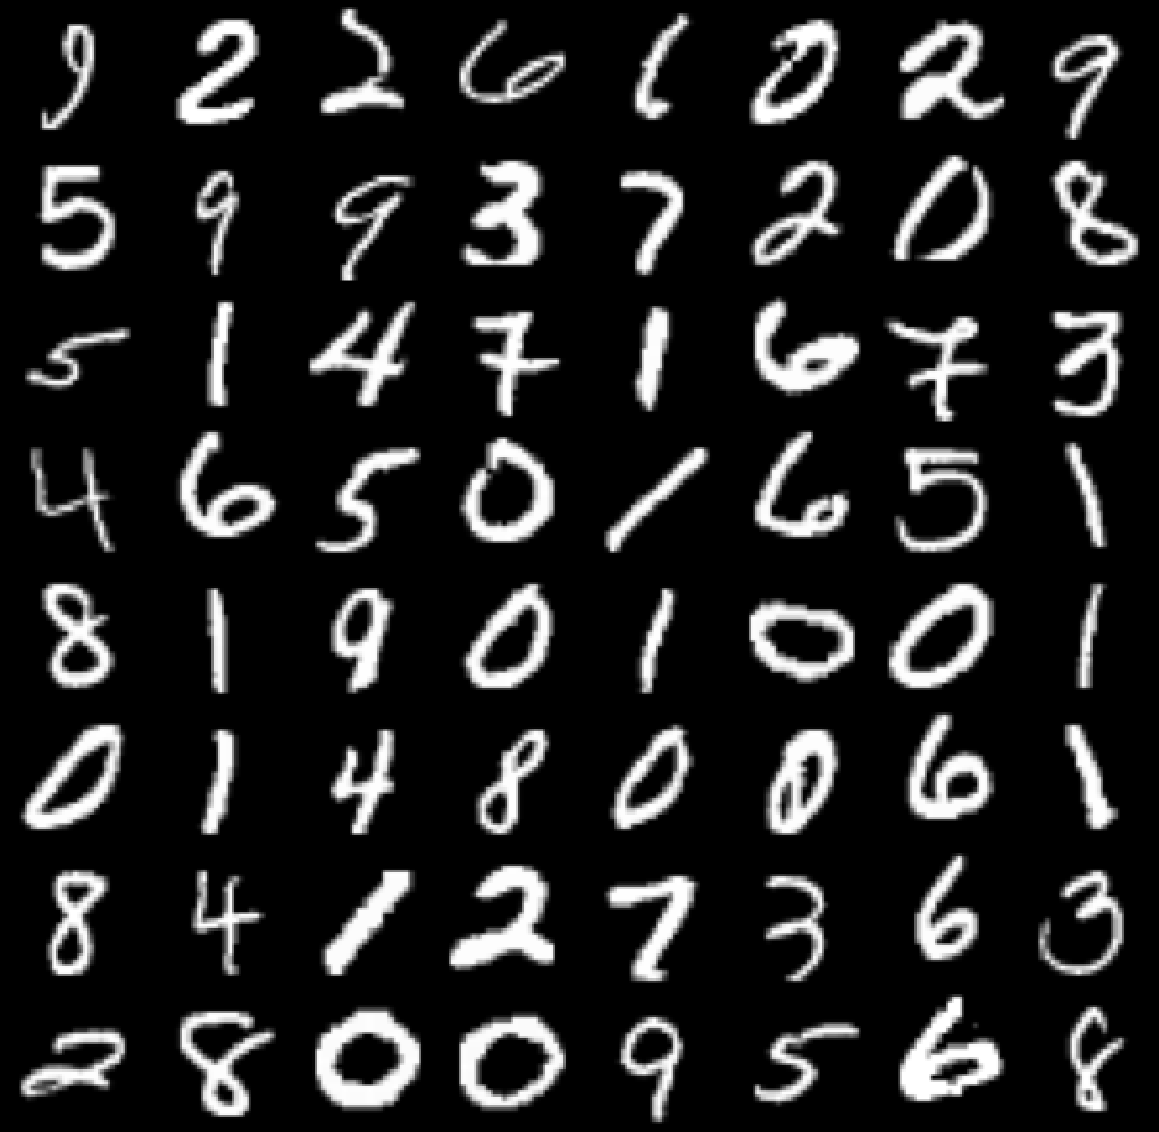
\includegraphics[width=0.4 \textwidth]{resources/minist_dataset.pdf}
		\caption{датасет рукописних цифр MNIST}
		\label{fig:minist_dataset}
	\end{figure}

	
	\section{Тренування моделі}
	\label{sec:model}
	У створені ефективної моделі машинного навчання велику роль грає не тільки обраний алгоритм, але й правильна обробка даних та використання методів оптимізації. Тому під час реалізації мультикласової логістичної регресії, також були застосовані декілька алгоритмів оптимізації.
	
	\subsection{Обробка даних}
	Значення зображень датасету MINIST знаходяться в проміжку $[0, 255]$, а для того щоб процес навчання відбувався швидше, необхідно щоб всі дані перебували в деякому малому проміжку, наприклад, такому як $[0, 1]$. Для цього можна скористатись методом нормалізації або стандартизації даних, але через те, що всі оригінальні значення знаходяться у фіксованому проміжку, найпростішим підходом буде просто розділити всі значення на максимальне число, тобто на $255$.

	\subsection{Оптимізація моделі}
	\subsubsection{Mini batch gradient descent}
	\noindent
	Для покращення роботи моделі будемо використовувати градієнтний спуск з mini batch  оптимізацією. Ідея даної оптимізації полягає в тому, щоб розбити весь тренувальний датасет на деяку кількість частин розміру $k$ $(k=2^{q}, q \in  \mathbb{N})$
	\begin{align*}
	&X = [X^{1}, X^{2}, ..., X^{|m/k|}]\\
	&Y = [Y^{1}, Y^{2}, ..., Y^{|m/k|}]
	\end{align*}
	
	Таким чином, ми будемо оновлювати параметри моделі $\omega$ і $b$ після обчислення функції втрати на кожній з цих частин, а не на всіх прикладах одразу. Перевага цього методу в тому, що він дає можливість за меншу кількість ітерацій досягти збіжності. Також його варто використовувати для того щоб зменшити обчислювальні ресурси необхідні для тренування моделі.

	\subsubsection{Momentum}
	\noindent
	Ще одним ефективним алгоритмом оптимізації є momentum оптимізація яка базується на методі рухомого середнього значення. Тепер під час оновлення ваг і зсуву моделі ми будемо враховувати і всі попередні обчислені градієнти теж, з деяким коефіцієнтом згладжування $\mu$. Оновлення параметрів моделі тепер буде виглядати наступним чином:
	\begin{align*}
		&V_{d\omega} = \mu V_{d\omega} + (1 - \mu) d\omega; \quad 
		\omega = \omega - \alpha V_{d\omega}; \\
		&V_{db} = \mu V_{db} + (1 - \mu) db; \; \; \quad
		b= b - \alpha V_{db}; 
	\end{align*}
	В результаті застосування цього методу, кроки градієнтного спуску будуть згладжені, що допоможе під час тренування уникати потрапляння моделі у точки локального оптимума.
	
	\subsection{Тренування}
	Для знаходження оптимальних гіперпараметрів моделі був використаний алгоритм перебору параметрів з заданої множини. За результатами перевірки на тестовому датасеті точність отриманої моделі складає $\sim 92\%$.
	
	% ============================================ %
	
	% ============================================ %
	\chapter{Методи атак}
	В цьому розділі будуть розглянуті деякі методи генерування змагальних зразків, які були реалізовані і протестовані на лінійній моделі натренованій в розділі \ref{sec:model}.
	
	Далі, під час опису будуть використовуватись такі позначення:
	\begin{itemize}
		\item $\boldsymbol{X}$ - це зображення, зазвичай це 3-D тензор (ширина $\times$ висота $\times$ глибина). В нашому випадку має розміри $(28 \times 28 \times 1)$ пікселів, яке складається з додатних цілих чисел в межах $[0, 255]$.
		\item $\boldsymbol{X}^{*}$ - згенерований змагальний приклад для зображення $\boldsymbol{X}$
		\item $y_{true}$ - правильний клас для зображення $\boldsymbol{X}$.
		\item $J(\boldsymbol{X}, y)$ - штрафна функція моделі. Ваги моделі $\omega$ навмисно не будемо вказувати, вважатимемо їх сталими, як значення які будуть отримані з моделі машинного навчання. В нашому випадку штрафною функцією є функція кросс-ентропії \ref{eq:cross-entropy}. 
		\item $Clip_{\boldsymbol{X}, \varepsilon} \{ \boldsymbol{X}^{*} \}$ - функція яка виконує по-піксельне обрізання зображення $X^{*}$ так, щоб результат був в $L_{\infty}$ $\varepsilon $ - околі вхідного зображення $\boldsymbol{X}$. Рівняння для цього виглядає наступним чином:
		
		\begingroup
		\setlength{\abovedisplayskip}{0pt}
		\setlength{\belowdisplayskip}{0pt}
		\begin{align}
		\label{eq:clip}
		\resizebox{.9 \textwidth}{!} 
		{
			$
			Clip_{X, \varepsilon} \{ \boldsymbol{X}^{*} \}(x, y, z) = 
			min\Big\{ 255, \boldsymbol{X}(x, y, z) + \varepsilon, max \{ 0, \boldsymbol{X}(x, y, z) - \varepsilon, \boldsymbol{X}^{*}(x, y, z) \} \Big\}
			$,
		}
		\end{align}
		\endgroup

		де $\boldsymbol{X}(x, y, z)$ - це значення каналу $z$ зображення $\boldsymbol{X}$ з координатами $(x, y)$.
	\end{itemize}

	\section{FGSM}
	Одним з найпоширеніших методів для генерування змагальних зразків машинного навчання є Fast Gradient Sign Method. Вперше він був представлений в роботі \textcite{goodfellow2014explaining}. Ідея цього методу полягає в тому, щоб знайти такий змагальний приклад $x^{*}$ який максимізує функцію втрати $J(x^{*}, y)$ до певного $L_{\infty}$ обмеження. Цього можна досягти один раз використавши зворотне поширення:
	\begin{equation}
	X^{*} = X + \varepsilon \cdot sign(\Delta_x J(x, y)),
	\end{equation}
	де $\varepsilon$ - деякий гіперпараметер.
	
	Для того щоб застосувати цей метод для логістичної регресії необхідно обчислити градієнт від функції кросс-ентропії \ref{eq:cross-entropy}. Для цього спочатку знайдемо похідну від $softmax$ функції:
	\begin{align*}
		z_i = \omega\tran x\ith + b; \quad
		\hat{y}_i = a_i = softmax(z_i); \quad
		softmax(z_i) = \frac{e^{z_i}}{\sum_{k=1}^{C} e_k^z}; \quad
	\end{align*}
	Якщо $i = j$,
	\begin{align}
	    \pdv{\hat{y_i}}{z_j} 
	    &=
	    \pdv{\frac{e^{z_i}}{\sum_{k=1}^{C} e_k^z}}{z_j} 
	    =
	    \frac{e^{z_i} \sum_{k=1}^{C} e^{z_k} - e^{z_j} e^{z_i}}{(\sum_{k=1}^{C}  e^{z_k})^2} 
	    = \\& =
	    \frac{e^{z_j}}{\sum_{k=1}^{C}  e^{z_k}} \times \frac{(\sum_{k=1}^{C} e^{z_k} - e^{z_j})}{\sum_{k=1}^{C}  e^{z_k}} 
	    = 
	    y_i(1-y_j)
	\end{align}
	Якщо $i \neq j$,
	\begin{align}
		\pdv{\hat{y_i}}{z_j}
		&=
		\pdv{\frac{e^{z_i}}{\sum_{k=1}^{C} e_k^z}}{z_j} 
		=
		\frac{0 - e^{z_j} e^{z_i}}{\sum_{k=1}^{C}  e^{z_k}} \times \frac{e^{z_i}}{\sum_{k=1}^{C} e^{z_k}} 
		= 
		-y_i y_j 
	\end{align}
	
	\begingroup
	\setlength{\abovedisplayskip}{0pt}
	\setlength{\belowdisplayskip}{0pt}
	
	Далі обчислюємо похідну від функції кросс-ентропії:
	\begin{align*}
		\xi(y, x) = - \sum_{i=1}^{C} y_j  \log (\hat{y_j})
	\end{align*}

	\begin{align*}
		\pdv{\xi}{z_i} 
		&= 
		- \sum_{j=1}^{C} \pdv{ y_j \log (\hat{y_j})}{z_i} 
		=
		- \sum_{j=1}^{C} y_j \pdv{ \log (\hat{y_j})}{z_i} 
		= 
		- \sum_{j=1}^{C} y_j \frac{1}{\hat{y_i}} \cdot \pdv{\hat{y_i}}{z_i} 
		= \\& =
		- \frac{y_i}{\hat{y_i}} \pdv{\hat{y_i}}{z_i} - \sum_{j \neq i} \frac{y_j}{\hat{y_j}} \pdv{\hat{y_j}}{z_i} 
		= 
		-\frac{y_i}{\hat{y_i}} \hat{y_i} (1 - \hat{y_i}) - \sum_{j \neq i} \frac{y_j}{\hat{y_j}} (-\hat{y_i} \hat{y_j}) 
		= \\& =
		-y_i + y_i \hat{y_i} + \sum_{j \neq i} y_j \hat{y_i}
		= 
		-y_i + \sum_{j=1}^{C} y_j \hat{y_i} 
		=
		\hat{y_i} - y_i ,
	\end{align*}
	\endgroup
		де i = 1, ..., C
		\newline	
		Тепер можна обчислити градієнт від штрафної функції по $x$:
		\begin{align}
		\pdv{\xi}{x_i} 
		&=
		\pdv{\xi}{z_i} \pdv{z_i}{x_i} 
		=
		(\hat{y_i} - y_i) \pdv{(\omega\tran x_i+ b)}{x_i} 
		=
		(\hat{y_i} - y_i) \omega\tran 
		=
		dz \cdot \omega\tran
	\end{align}
	 Маючи всі наведені обчислення, можна записати алгоритм знаходження змагального прикладу \ref{alg:fgsm}.
	\begin{algorithm}
		\caption{$FGSM$}
		\label{alg:fgsm}
		\begin{algorithmic}[1]
			\State \algorithmicrequire{Приклад $x$, клас $y_{true}$, класифікатор $f$, параметри: $\omega, b$.}
			\State \algorithmicrequire{значення пертурбації $\varepsilon$.}
			\State \algorithmicensure{ Adversarial $x^{*}$ з нормою $\|x^{*} - x\|_{\infty} \leq \varepsilon $;}
			\State $z = \omega\tran x + b$;
			\State $\hat{y} = softmax(z)$;
			\State $\delta = (\hat{y} - y_{true}) \cdot \omega\tran$;
			\State $x^{*} = Clip_{X, \varepsilon} \big\{ x + \alpha \cdot sign( \delta ) \big\}$;
			\State \algorithmreturn{$x^{*} = x^{*}_{T}$}.
		\end{algorithmic}
	\end{algorithm}
	
	\section{I-FGSM}
	Даний метод є модифікацією попереднього, особливість якого полягає в тому, що для знаходження змагального прикладу буде використовуватись ітераційний підхід.	Ми застосовуємо звичайний метод декілька разів з певним невеликим кроком $\alpha$ і після кожного кроку використовуємо функцію $clip$ \ref{eq:clip}, для того щоб переконатись що значення знаходяться в $\varepsilon$-околі оригінального зображення.
	
	Ітераційний алгоритм швидкого градієнтного спуску буде мати вигляд \ref{alg:i-fgsm}.
	\begin{algorithm}
		\caption{$I-FGSM$}
		\label{alg:i-fgsm}
		\begin{algorithmic}[1]
			\State \algorithmicrequire{Приклад $x$, значення класу $y_{true}$, класифікатор $f$}
			\State \algorithmicrequire{значення пертурбації $\varepsilon$, кількість ітерації $T$.}
			\State \algorithmicensure{ Adversarial $x^{*}$ з нормою $\|x^{*} - x\|_{\infty} \leq \varepsilon $;}
			\State $\alpha = \varepsilon / T $;
			\State $x^{*} = x$;
			\For{$t=0 \; to \; T-1$}
			\State $x^{*} = Clip_{X, \varepsilon} \big\{ x^{*} + \alpha \cdot  sign(\Delta_x J(x, y)) \big\}$;
			\EndFor
			\State \algorithmreturn{$x^{*} = x^{*}_{T}$}.
		\end{algorithmic}
	\end{algorithm}
	
	Результат роботи алгоритму для $\varepsilon = 0.05$ можна побачити на рисунку \ref{fig:i-fgsm-example}.
	\begin{figure}[h]
		\centering
		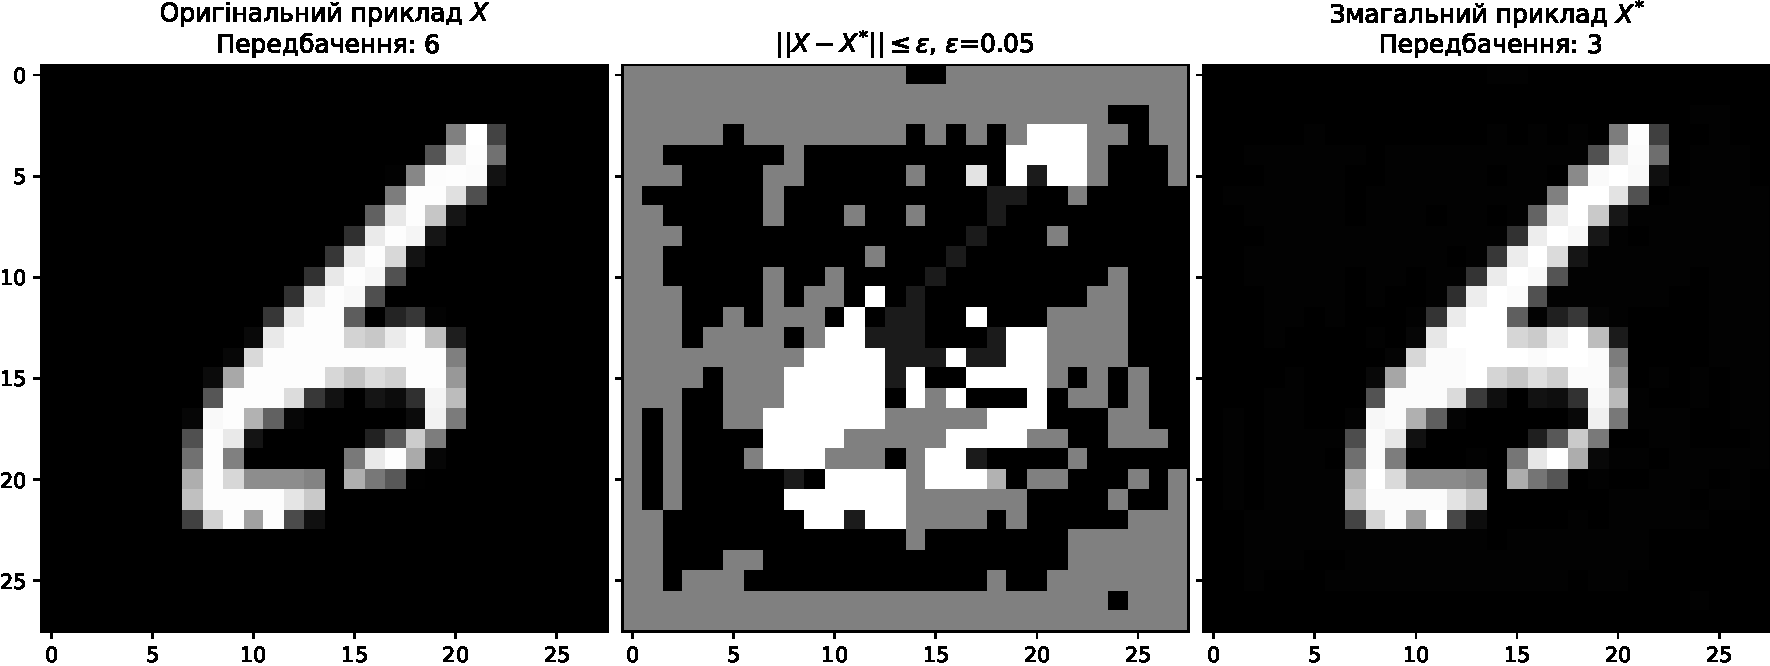
\includegraphics[width=0.9\textwidth]{resources/i-fgsm-example.pdf}
		\caption{}
		\label{fig:i-fgsm-example}
	\end{figure}
		
	\newpage
	\section{TI-FGSM}
	TI-FGSM або як його ще називаюсь Projected Gradient Descent є цілеспрямованою версією попереднього алгоритму, а отже він дає можливість обрати клас який має передбачити модель. Два попередні методи описані вище намагалися максимізувати функцію втрати для правильного класу, не вказуючи яким буде неправильний клас. Цей метод - навпаки, мінімізує функцію втрати для деякого заданого неправильного класу. На сам алгоритм це вплине так, що тепер під час градієнтного спуску ми будемо рухатись в напрямку, протилежному градієнту штрафної функції, тобто на етапі додавання пертурбацій у вхідний приклад, знак буде змінений на протилежний.
	%[\ref{alg:ti-fgsm}].

	%\begin{algorithm}
	%	\caption{$TI-FGSM$}
	%	\label{alg:ti-fgsm}
	%	\begin{algorithmic}[1]
	%		\State \algorithmicrequire{Приклад $x$, значення класу $y_{true}$, класифікатор $f$}
	%		\State \algorithmicrequire{значення пертурбації $\varepsilon$, кількість ітерації $T$.}
	%		\State \algorithmicensure{ Adversarial $x^{*}$ з нормою $\|x^{*} - x\|_{\infty} \leq \varepsilon $;}
	%		\State $a = \varepsilon / T $;
	%		\State $x^{*} = x$;
	%		\For{$t=0 \; to \; T-1$}
	%		\State $x^{*} = Clip_{X, \varepsilon} \big\{ x^{*} - \alpha \cdot  sign(\Delta_x J(x, y)) \big\}$;
	%		\EndFor
	%		\State \algorithmreturn{$x^{*} = x^{*}_{T}$}.
	%	\end{algorithmic}
	%\end{algorithm}

	\section{MI-FGSM}	
	Попередні розглянуті методи хоч і є ефективними, але мають певні недоліки.
	Для прикладу однокроковий (FGSM) обчислює градієнт тільки один раз, припускаючи, що межа рішень є лінійною. На практиці це зазвичай не так і тому для змагального прикладу, згенерованого таким чином, характерне \textit{недотренування} що обмежує ефективність атаки. З іншого боку ітераційний метод (I-FGSM), з кожною ітерацією жадібно рухає змагальний приклад в напрямку градієнту, що може призвести до зупинки в локальній точці оптимума та \textit{перетренуванню} моделі. Щоб розв'язувати цю проблему в роботі \textcite{dong2017boosting} була представлена momentum оптимізація ітераційного методу. Вона допомагає стабілізувати напрямок зміни прикладу що допомагає уникнути потрапляння в локальному оптимумі.
	
	Алгоритм даної модифікації має наступний вигляд \ref{alg:mi-fgsm}	
	\begin{algorithm}
		\caption{$MI-FGSM$}
		\label{alg:mi-fgsm}
		\begin{algorithmic}[1]
			\State \algorithmicrequire{Приклад $x$, значення цілі y, класифікатор $f$.};
			\State \algorithmicrequire{значення пертурбації $\varepsilon$, значення цілі y, кількість ітерації $T$.};
			\State \algorithmicensure{ Adversarial $x^{*}$ з нормою $\|x^{*} - x\|_{inf} \leq \varepsilon $};
			\State $a = \varepsilon / T$;
			\State $g0 = 0;$ $x^{*}_0 = x$;
			\For{$t=0 \quad to \quad T-1$}
			\State $g_{t+1} = \mu \cdot g_t + \frac{\Delta_x J(x^{*}, y)}{\|\Delta_x J(x^{*}, y)\|_1}$;
			\State $x^{*} = Clip_{X, \varepsilon} \big\{ x^{*}_{t} + \alpha \cdot sign(g_{t+1}) \big\}$;
			\EndFor
			\State \algorithmreturn{$x^{*} = x^{*}_{T}$}.
		\end{algorithmic}
	\end{algorithm}
	
	\section{DeepFool}
	DeepFool була вперше представлена в роботі \textcite{moosavidezfooli2015deepfool}. На відмінно від FGSM методу цей алгоритм не можна використовувати для цілеспрямовиних атак, де є можливість вибрати клас який має передбачити модель. Отже, його можна використовувати тільки для генерування прикладів які будуть класифікуватись хибно. Основною метою цього методу є знаходження мінімального необхідного значення пертурбації, для того, щоб модель хибно передбачила клас прикладу.
	
	\begin{figure}[h]
		\centering
		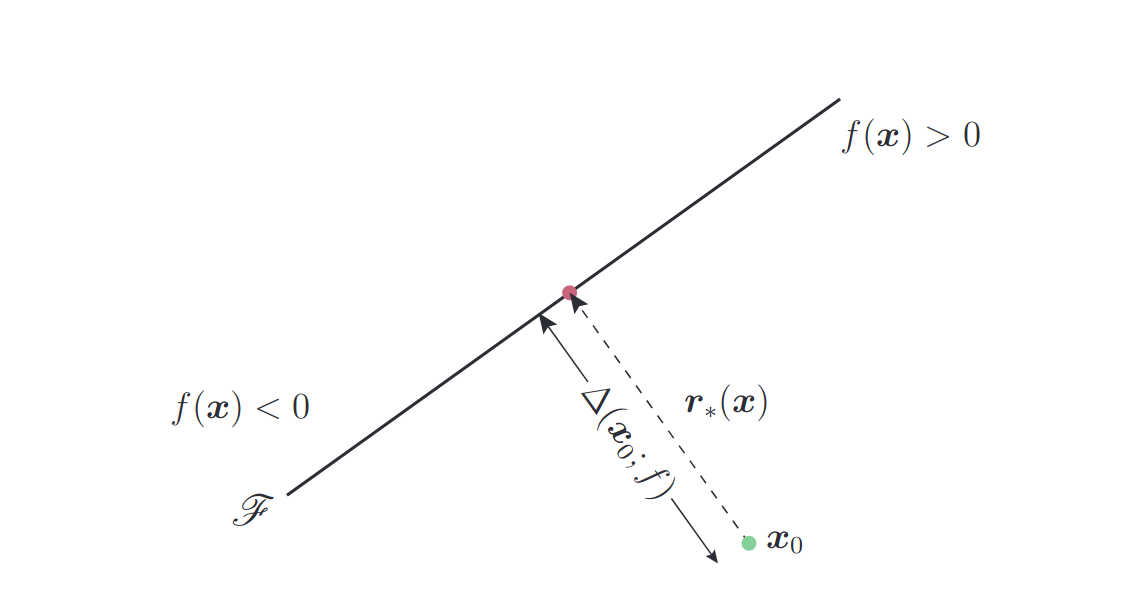
\includegraphics[width=\textwidth]{resources/deepfool.jpg}
		\caption{Приклад для лінійного бінарного класифікатора \cite{moosavidezfooli2015deepfool}}
		\label{fig:dfhyperline}
	\end{figure}

	Для випадку бінарної класифікації легко бачити, що надійність моделі $f$ в точці $ x_{0}, \; \Delta(x_{0}; f)$, дорівнює відстані від $x_{0}$ до площини гіперпараметра $\mathscr{F} = \{ x: \omega\tran x + b = 0 \}$, яка розділяє два класи (Рис. \ref{fig:dfhyperline}). Таким чином, мінімальний зсув, необхідний для зміни рішення класифікатора відповідає ортогональній проєкції $x_{0}$ на $\mathscr{F}$. Це можна записати у вигляді формули:
	\begin{align}
		r_{*}(x_{0}) := -\frac{f(x_{0})}{\norm{\omega}_{2}^{2}} \omega .
	\end{align}
	
	Для того що реалізувати цей алгоритм необхідно спочатку знайти градієнт від функції кросс-ентропії \ref{eq:cross-entropy} по $x$.
	\begin{equation}
	\pdv{\hat{y_i}}{x_k}  =
	\begin{cases}
	y_i(1-y_j) & \text{, якщо $i = j$}\\
	- y_i y_j & \text{, якщо $i \neq j$}\\
	\end{cases}
	\; \text{, де} \quad i = 1, .. ,C; \; j = 1, .. ,C;
	\end{equation}
	
	При знаходженні похідної нас цікавить випадок $i = j$, тому отримуємо:
	\begin{align*}
	\pdv{\hat{y_i}}{x_k} 
	&=
	\pdv{\hat{y_i}}{z_j} \pdv{z_j}{x_k} 
	=
	y_i(1-y_i) \pdv{(\omega\tran x_k + b)}{x_k} 
	=
	y_i(1-y_i) \omega\tran 
	=
	dz \cdot \omega\tran
	\end{align*}
	Для випадку $l_2$ норми DeepFool алгоритм для мультикласового випадку буде мати наступний вигляд \ref{alg:deepfool}.
	\begin{algorithm}
		\caption{DeepFool: мультикласовий випадок}
		\label{alg:deepfool}
		\begin{algorithmic}[1]
			\State \algorithmicrequire{Приклад $x$, значення цілі y, класифікатор $f$.};
			\State \algorithmicrequire{значення цілі y, кількість ітерації $T$.};
			\State \algorithmicensure{ Adversarial $x^{*}$ з нормою $\|x^{*} - x\|_{2} \leq \varepsilon $};
			\State $x_0 = x$; $i = 0$; 
			\While{$\hat{f}(x_i) = \hat{f}(x_0) $}
				\For{$k \neq \hat{f}(x_0)$}
					\State $ w_{k}' = \Delta f_k(x_i) - \Delta f_{\hat{k}(x_0)} (x_i)$;
					\State $ f_{k}' = \Delta f_k(x_i) - \Delta f_{\hat{k}(x_0)} (x_i)$;
				\EndFor
				\State $\hat{l} = \arg \min_{k \neq \hat{f}(x_0)} \frac{\abs{f_{k}'}}{\|w_{k}'\|_2}$;
				\State $r_i = \frac{\abs{f_{\hat{l}}'}}{\|w_{\hat{l}}'\|_{2}^{2}} w_{\hat{l}}'$;
				\State $x_{i+1} = x_i + r_i$;
				\State $i = i + 1$;
			\EndWhile
			\State \algorithmreturn{$\hat{r} = \sum_{i} r_i $}.
		\end{algorithmic}
	\end{algorithm}
	\\	
	Результат роботи алгоритму для $\varepsilon = 0.05$ можна побачити на рисунку \ref{fig:i-fgsm-example}.
	\begin{figure}[h]
		\centering
		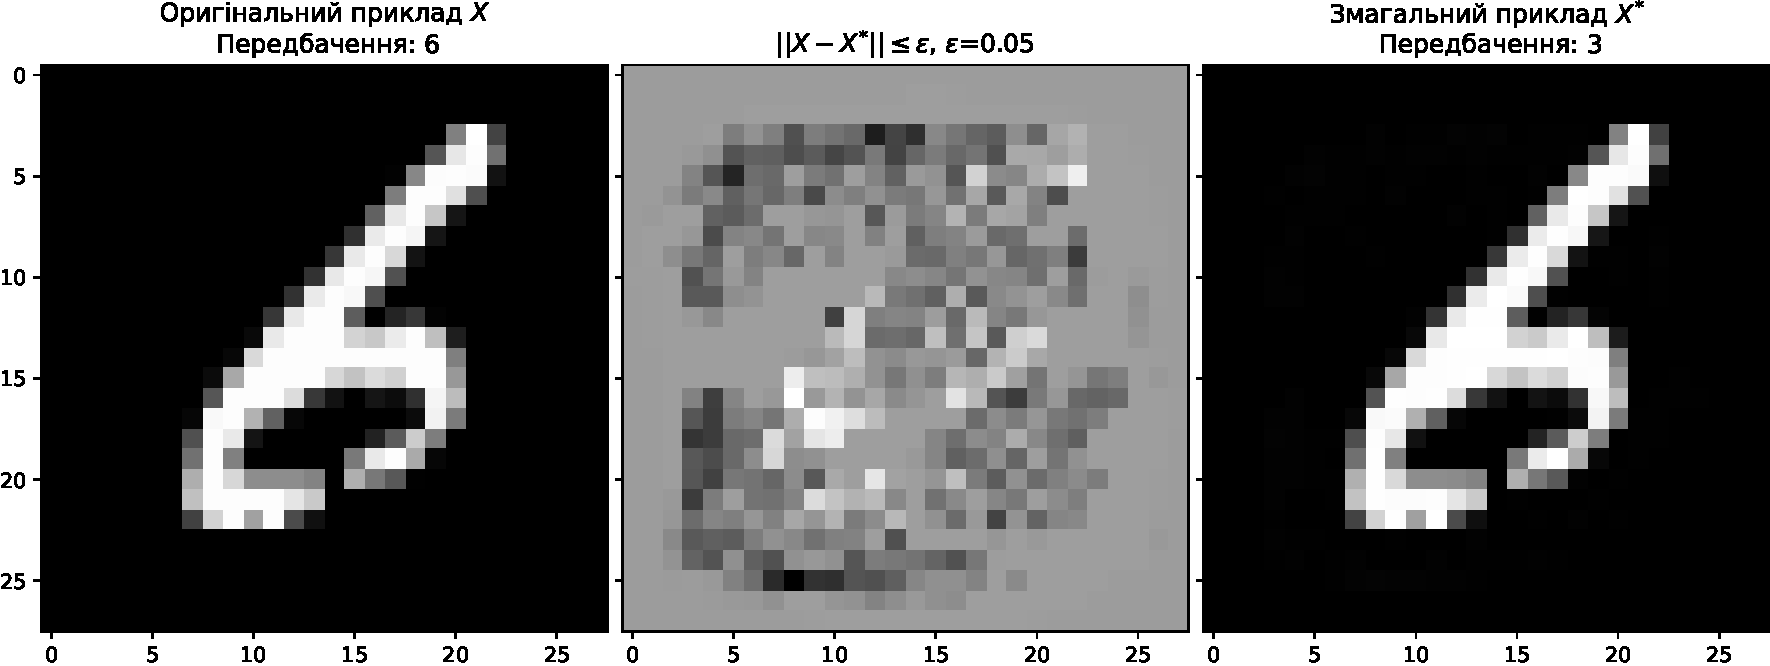
\includegraphics[width=1\textwidth]{resources/deepfool-example.pdf}
		\caption{}
		\label{fig:deepfool-example}
	\end{figure}
	
	% ============================================ %	
	\chapter{Методи захисту}
	Маючи класифікатор моделі $F$ і деяке зображення $\hat{X}$, яке може бути або оригінальним зображенням $X$ або змагальним $X^{*}$, метою захисту моделі є або посилити $F$ як $F'$ таким чином, щоб $F(\hat{X}) = F(X)$, або трансформувати $\hat{X}$ через деякий метод $T$ так, щоб $F(T(\hat{X})) = F(X)$.
	
	\section{Randomization}
	Одним методів захисту, який добре продемонстрував себе в ході змагань за найкращих метод атак та захисту 2018 року \cite{kurakin2018adversarial} є рандомізація вхідних даних.
	
	Зазвичай пертурбації, які генеруються в наслідок ітераційних атак, можуть легко опинитись перетренованими для деяких параметрів моделі та є унікальними для них. Ця властивість дає можливість зробити висновок, що трансформації додані до вхідних даних, такі як зміна розміру, стискання, або додавання відступів до зображення може зруйнувати структуру певної змагальної пертурбації і таким чином стати непоганим захистом. Якщо трансформації відбуваються випадково і нападник не знає їх характер, тоді цей метод може стати ефективним як для атак на закриті моделі, так і на відкриті теж.
	Алгоритм для даного методу буде мати наступний вигляд:
	
	\begin{enumerate}
	\item Спочатку оригінальне зображення $x$ розмірами $W \times H \times 1$ замінюють на нове $x'$ з випадково вибраними розмірами $W' \times H' \times 1$. Ватро зауважити, що $|W' - W|$ та $|H' - H|$ мають бути у відносно малому проміжку, інакше точність моделі на чистих зображеннях суттєво впаде.
	\item Другим кроком буде випадкове наповнення деякого простору навколо зображення $x'$ нулями, після чого буде утворене нове зображення $x''$ з розмірами $W'' \times H'' \times 1$. Таким чином ми можемо наповнити зображення $w$ нульовими пікселями зліва, $W'' - W' - w$ нульовими пікселями справа, $h$ зверху та $H'' - H' - h$ зліва. Це в результаті дає нам  $(W''-W'+1) \times (H''- H'+1)$ різних варіацій.
	\item Після двох попередніх етапів, зображення $x''$ передається оригінальному класифікатору натренованої моделі.
	\end{enumerate}

	\section{Pixel Reflection}
	Ще одним методом, який за допомогою внесення деякого шуму в зображення намагається зруйнувати його змагальну структуру є Pixel Reflection. Він був представлений в роботі \textcite{prakash2018deflecting} і добре продемонстрував себе в захисті нейронних мереж. Ідея методу полягає в тому, щоб випадково вибрати піксель із зображення і потім, так само випадково замінити його на інший піксель в його малому околі. 
	
	Для того щоб покращити цей алгоритм можна визначити найбільш важливі для класифікації класів місця зображення і уникати їх деформації, знижуючи ймовірність внесення туди змін. Для цього можна скористатись активаційною картою класів моделі. Для випадку нашої моделі вони будуть мати вигляд \ref{fig:classactivationmap}.
	\begin{figure}[h]
		\centering
		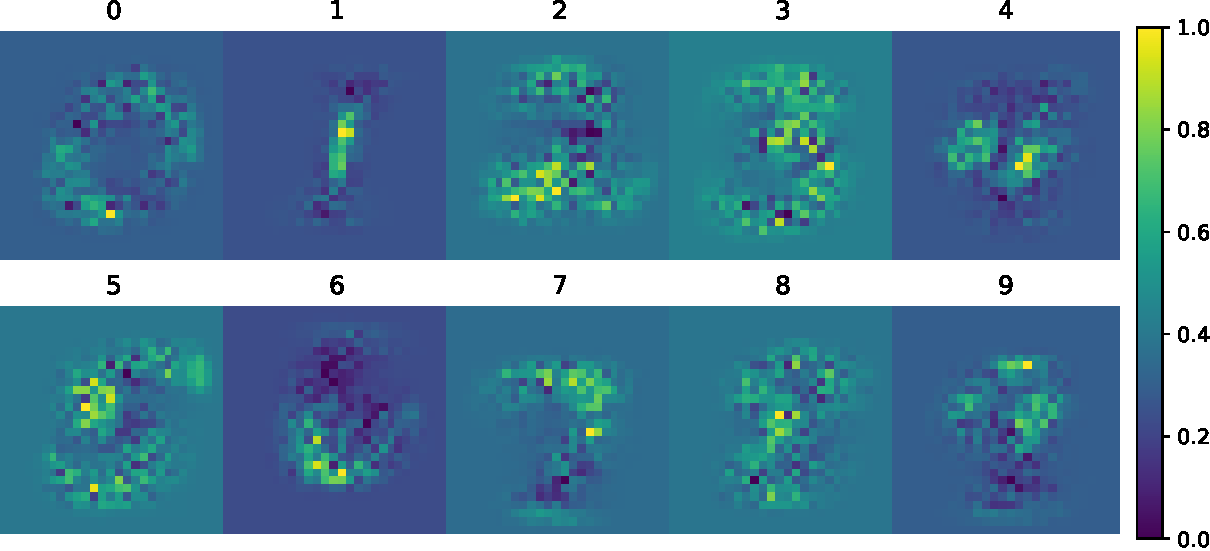
\includegraphics[width=\textwidth]{resources/classactivationmap.pdf}
		\caption{}
		\label{fig:classactivationmap}
	\end{figure}

	Загалом, для захисту конкретного прикладу нас цікавить карта класу, якому модель надає найвищу ймовірність. Однак, враховуючи те, що серед вхідної інформації будуть потрапляти змагальні приклади, клас який буде визначатись як найбільш ймовірний, скоріше за все буде неправильним. На щастя, змагальний приклад який змінює найімовірніший клас, зазвичай майже ніяк не впливає на всі інші. За результатами експериментів, можна сказати, що в переважній більшості випадків модель визначає змагальний приклад другим за ймовірністю класом для оригінального зображення. Тому для того щоб уникати пошкоджень зображення в найважливіших для класифікації місцях, будемо використовувати середнє значення активаційних карт для двох найімовірніших класів.
	

	% ============================================ %	
	\chapter{Аналіз алгоритмів}
	Для побудови графіків з високою точністю, але оптимально з точки зору використання обчислювальних ресурсів, для отримання результатів по роботі алгоритмів атак та захисту використовувались 1 тис. зображень з тестового датасету, які були нормалізовані і тому складались зі значень в проміжку $[0, 1]$. Критерієм деформації прикладу буде використовуватись норма $L_{\infty}$ яка має бути меншою за максимальне значення пертурбації $\varepsilon$. Експерименти проводились для деякої кількості рівновіддалених значень $\varepsilon$:
	$$\varepsilon_{i}=a + i \cdot h, \quad h=\frac{b - a}{n}; \quad i=0,..,n; \quad n=30$$
	\section{Аналіз атак}
	
	\begin{figure}[!htb]
		\minipage[t]{0.49\textwidth}
		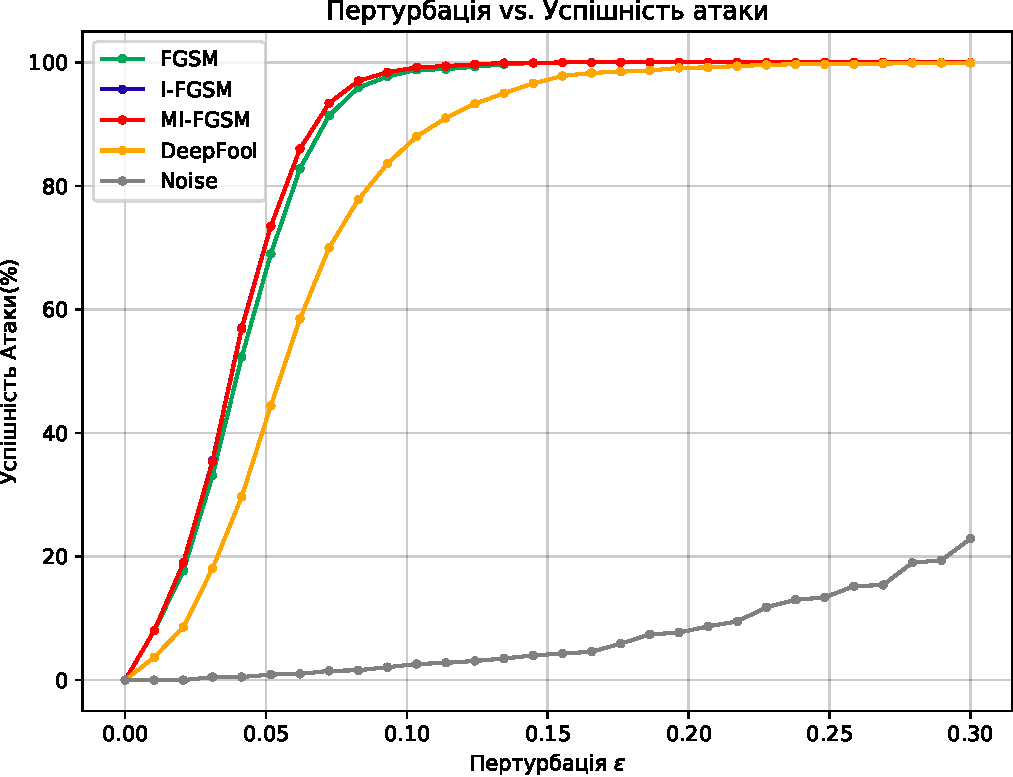
\includegraphics[width=1\textwidth]{resources/attacks_bench_8_6.pdf}
		\caption{Графік залежності успішності атаки від величини пертурбації. Нижньою межею буде виступати випадковий шум. }
		\label{fig:attacks_bench}
		\endminipage\hfill
		\minipage[t]{0.49\textwidth}
		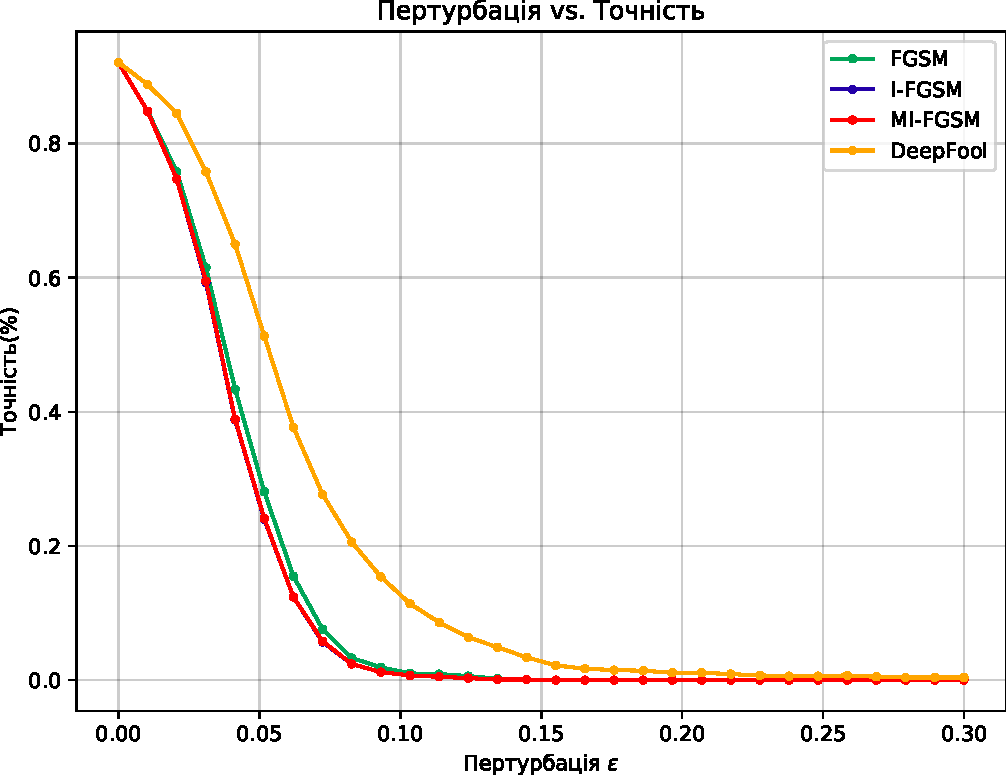
\includegraphics[width=1\textwidth]{resources/defenses_bench_8_6.pdf}
		\caption{Графік залежності успішності класифікації моделі від величини пертурбації. Початкова точність моделі \\ $\sim 92\%$}
		\label{fig:defenses_bench}
		\endminipage
	\end{figure}
	Під час побудування графіку залежності успішності атак від значення пертурбації \ref{fig:attacks_bench}, використовувались тільки такі тестові приклади, які коректно передбачались класифікатором $f$. У випадку графіка точності моделі \ref{fig:defenses_bench} брались випадково обрані приклади, серед яких були і ті, що визначались класифікатором хибно.
	
	Як можна побачити з графіків \ref{fig:attacks_bench} та \ref{fig:defenses_bench} класичний FGSM алгоритм відстає за ефективністю від його  ітераційних модифікацій. В той час як I-FGSM та MI-FGSM методи для даної моделі та датасету дають майже ідентичні результати. Попри те, що DeepFool алгоритм націлений на утворення змагальних прикладів з мінімальним рівнем деформації оригінального зображення, він опинився найслабкішим з точки зору $L_{\infty}$ норми. Однак зазвичай, приклади утворені за допомогою цього алгоритму мають меншу евклідову норму ніж в інших розглянутих алгоритмах і, відповідно, візуально вони є теж менш пошкодженими. 
	
	\section{Аналіз захисту}
	Для того щоб проаналізувати методи захисту використовувались оригінальні тестові зображення, а також зображення які були модифіковані певним алгоритмом захисту. Далі для обох множин прикладів застосовувались розглянуті атаки, після чого були побудовані порівняльні графіки.

	\subsubsection{Randomization}
	\noindent
	З наведених графіків \ref{fig:pixeldeflection} можна побачити, що алгоритм випадкової зміни розмірності опинився неефективним для захисту даної моделі. Хоча була перевірена велика кількість різних варіантів параметрів, знайти такі, щоб точність моделі залишалась на високому рівні так і не вдалось. Навіть при дуже малих деформаціях зображень, класифікатор починав передбачати їх суттєво гірше і точність моделі знижувалась.
	\begin{figure}[!htb]
		\minipage[t]{0.32\textwidth}
		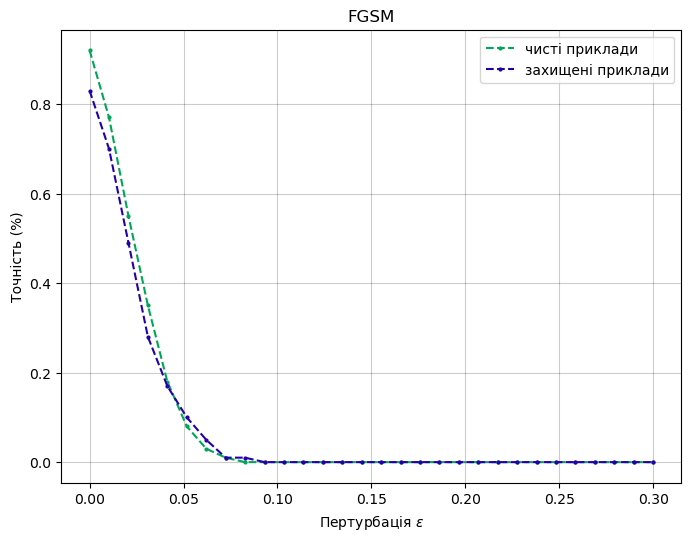
\includegraphics[width=1\textwidth]{resources/fgsm_rand_defence.png}
		\endminipage\hfill
		\minipage[t]{0.32\textwidth}
		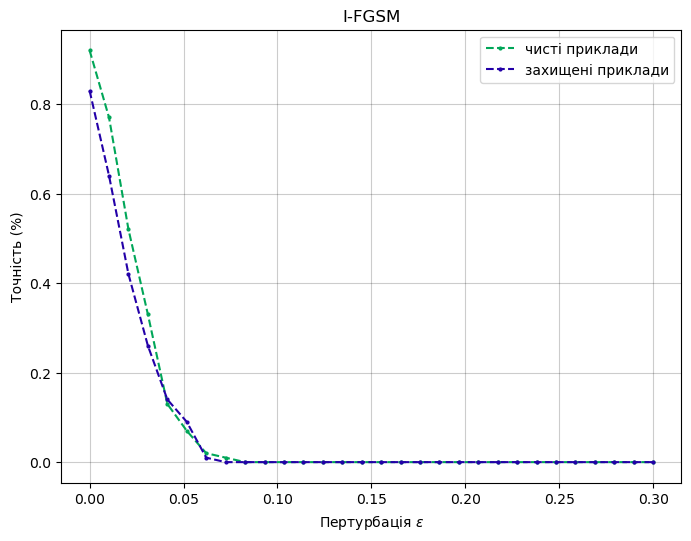
\includegraphics[width=1\textwidth]{resources/ifgsm_rand_defence.png}
		\endminipage
		\minipage[t]{0.32\textwidth}
		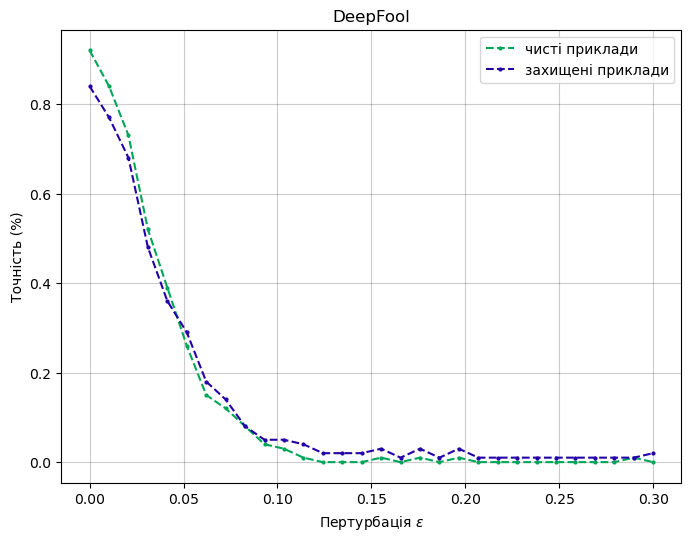
\includegraphics[width=1\textwidth]{resources/deepfool_rand_defence.png}
		\endminipage\hfill
		\caption{Randomization}
		\label{fig:randomization}
	\end{figure}
	% ============================================ %	

	\subsubsection{Pixel Deflection}
	\noindent
	Другий протестований метод захисту від атак на моделі машинного навчання продемонстрував себе значно краще ніж попередній. Навіть при відносно великій кількості зсунутих пікселів модель майже не втрачала точність. В результаті підбирання оптимальних параметрів для деформації вхідного зображення вдалось досягнути того, щоб при класифікації без генерування змагальних прикладів, тобто коли $\varepsilon=0$, точність моделі не падала зовсім \ref{fig:pixeldeflection}. Однак, використовуючи ці параметри успішність проведених атак знижувалась досить слабо. Тому попри те, що цей метод в правильних умовах ніяк не шкодить ефективності моделі, такий спосіб не можна вважати надійним захистом від атак.
	
	\begin{figure}[!htb]
		\minipage[t]{0.32\textwidth}
		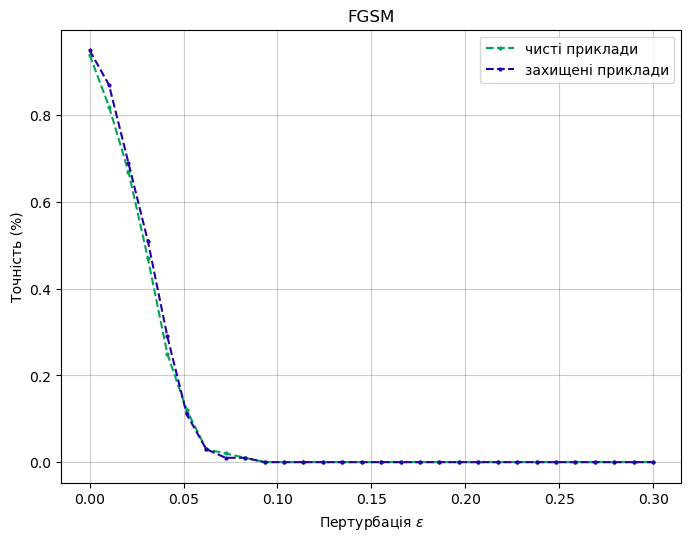
\includegraphics[width=1\textwidth]{resources/fgsm_defl_defence.png}
		\endminipage\hfill
		\minipage[t]{0.32\textwidth}
		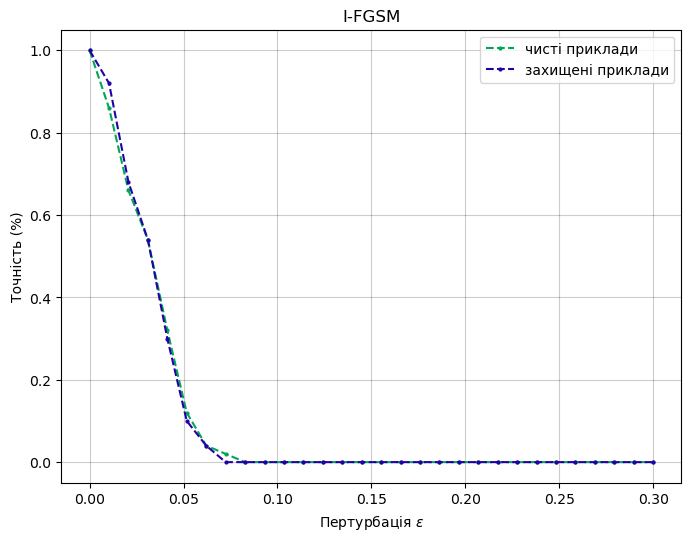
\includegraphics[width=1\textwidth]{resources/ifgsm_defl_defence.png}
		\endminipage
		\minipage[t]{0.32\textwidth}
		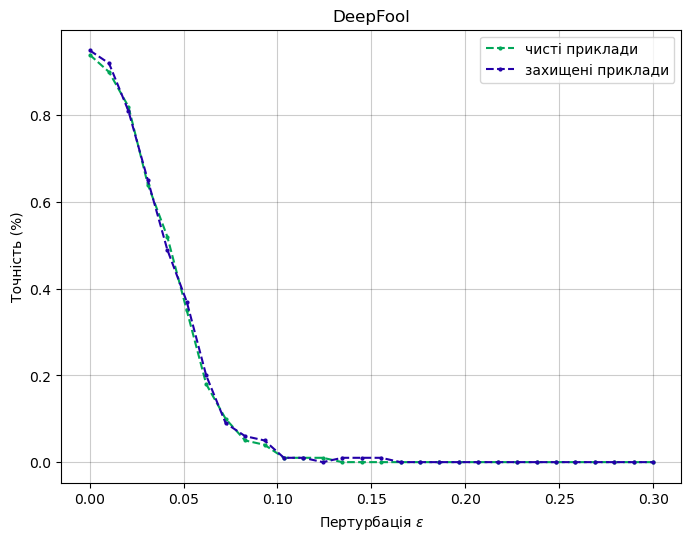
\includegraphics[width=1\textwidth]{resources/deepfool_defl_defence.png}
		\endminipage\hfill
		\caption{Pixel Deflection}
		\label{fig:pixeldeflection}
	\end{figure}
	
	Загалом можна зробити висновок, що методи захисту які базуються на ідеї випадкових деформацій зображень є не дуже ефективними у випадку лінійних моделей машинного навчання. Основна причина цього полягає в тому, що для того щоб захиститись від атак такими методами необхідно досить суттєво деформувати вхідне зображення, а через те що лінійні методи не здатні побудувати достатньо складні зв'язки між даними, вони є досить вразливі до такий деформацій. Отже, точність передбачення на деформованих зображеннях може падати досить швидко і такі методи захисту не можуть бути використані належним чином.

	\chapter{Висновок} 
	
	В результаті роботи була реалізована лінійна модель машинного навчання, на якій були проаналізовані декілька методів генерування змагальних прикладів. Серед них були розглянуті однокроковий алгоритм FGSM, його ітераційні варіації, а також DeepFool метод. В межах $L_{\infty}$ норми найефективнішими методами опинились ітераційна модифікація та momentum оптимізація алгоритму FGSM. Також були розглянуті два методи захисту які базуються на ідеї руйнування структури змагальних прикладів через додавання в зображення контрольованого шуму. За результатами експериментів, метод випадкової зміни розмірності зображення опинився неефективним для захисту лінійних моделей машинного навчання. Інший метод захисту Pixel Deflection стабільно зменшував ймовірність успішної атаки, але за отриманими результатами можна сказати, що він теж не є абсолютно надійним захистом від розглянутих методів атак.
	
	%============================================ %

	\nocite{goodfellow2014explaining}
	\nocite{kurakin2016adversarial}
	\nocite{moosavidezfooli2015deepfool}
	\nocite{dong2017boosting}
	\nocite{dong2019benchmarking}
	\nocite{yuan2017adversarial}
	\nocite{kurakin2018adversarial}
	\nocite{naseer2018local}
	\nocite{santhanam2018defending}
	\nocite{prakash2018deflecting}
	\printbibliography[title={Бібліографія}]
	% ============================================ %
\end{document}